\begin{figure}
\centering
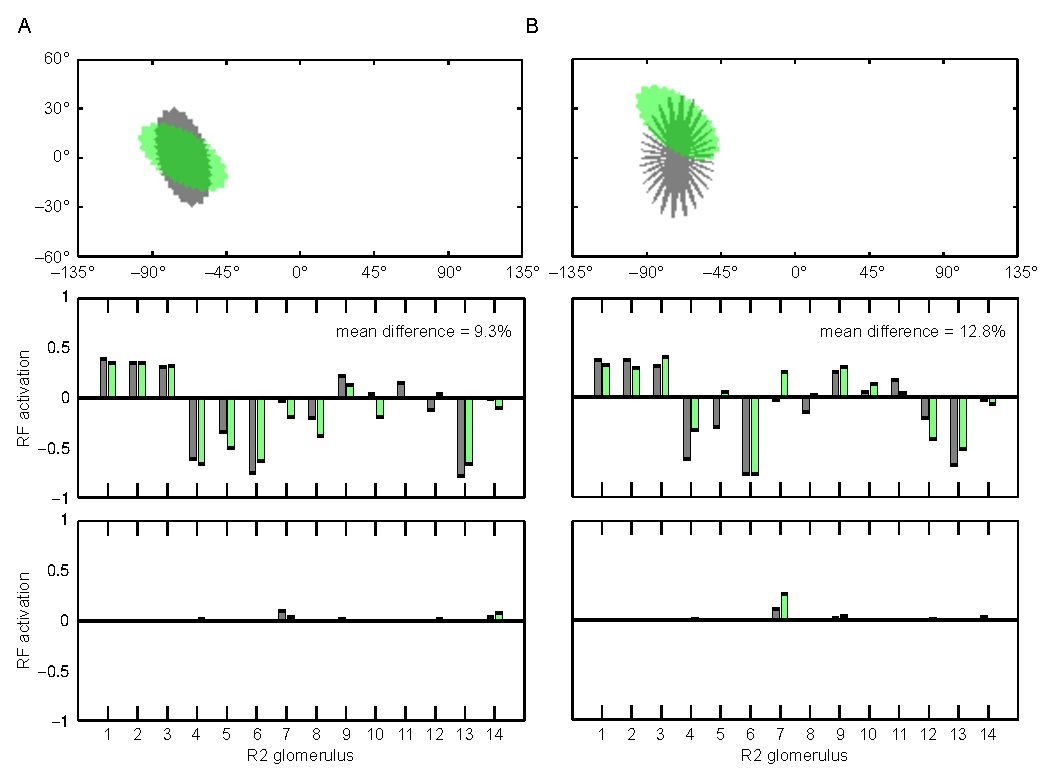
\includegraphics{figures/simdiff}
\caption{An example of two stimuli which appear very different, but yield similar responses from R2 \acp{RF} (\ac{rms} difference = 0.0144). The \ac{RF} of the R2 cells are superimposed. The stimuli are `blobs' of the form described in Section~\ref{sec:methods:stimuli} with vertical centres of mass at 0\degree and 20\degree. A Matlab optimisation is then run with \texttt{fminsearch} to find two blobs which produce a similar pattern of activation in the simulated R2 neurons (as determined by \ac{rms} difference).}

\label{supfig:fcp}
\end{figure}
